As constantes iniciais do modelo de motor apresentado no Capítulo~\ref{chap:modelagem} foram obtidas por ensaios estáticos em bancada dinamométrica, utilizando o motor empregado na aeronave (SunnySky A2212, $1000$~kV). A montagem e a operação da bancada, bem como as medições reunidas na Tabela~\ref{tab:bancada}, resultam do trabalho de \textcite{Diorio2026}, e foram aqui adotadas como ponto de partida do modelo de propulsão. Nos ensaios, para diferentes níveis de comando, mediram-se a velocidade angular do rotor, o empuxo e o contra-torque do conjunto motor e hélice, tomando-se a média de três repetições. As figuras a seguir apresentam os ajustes que fornecem o ganho $C_R$, a velocidade mínima $\Omega_b$ e os coeficientes de empuxo $c_T$ e de contra-torque $c_M$, refinados individualmente para cada um dos quatro motores no processo de identificação.

\begin{table}[ht]
\centering
\caption{Medições de bancada do conjunto motor e hélice (DIÓRIO, 2026).}
\label{tab:bancada}
\begin{tabular}{c c c c}
\toprule
$\delta_{PWM}$ [$\mu$s] & $\Omega$ [RPM] & $T$ [N] & $Q$ [N$\cdot$m] \\
\midrule
1000 & 0    & 0,00 & 0,000 \\
1167 & 2432 & 0,88 & 0,028 \\
1333 & 3378 & 1,81 & 0,058 \\
1500 & 4102 & 2,80 & 0,093 \\
1667 & 5087 & 4,40 & 0,134 \\
1833 & 5791 & 5,88 & 0,172 \\
2000 & 6063 & 6,79 & 0,176 \\
\bottomrule
\end{tabular}
\end{table}

A primeira etapa do modelo relaciona o comando normalizado $\sigma_i \in [0,1]$, definido por $\sigma_i = (\delta_{PWM,i}-\delta_{\min})/(\delta_{\max}-\delta_{\min})$ com $\delta_{\min}=1000~\mu$s e $\delta_{\max}=2000~\mu$s, à velocidade angular de regime permanente. Excluindo o ponto de motor parado, o ajuste linear por mínimos quadrados da Equação~\eqref{eq:motor-input} aos pontos medidos, apresentado na Figura~\ref{fig:ap-pwm-rpm}, fornece $C_R = 4523$~RPM e $\Omega_b = 1837$~RPM.

\begin{figure}[ht]
    \centering
    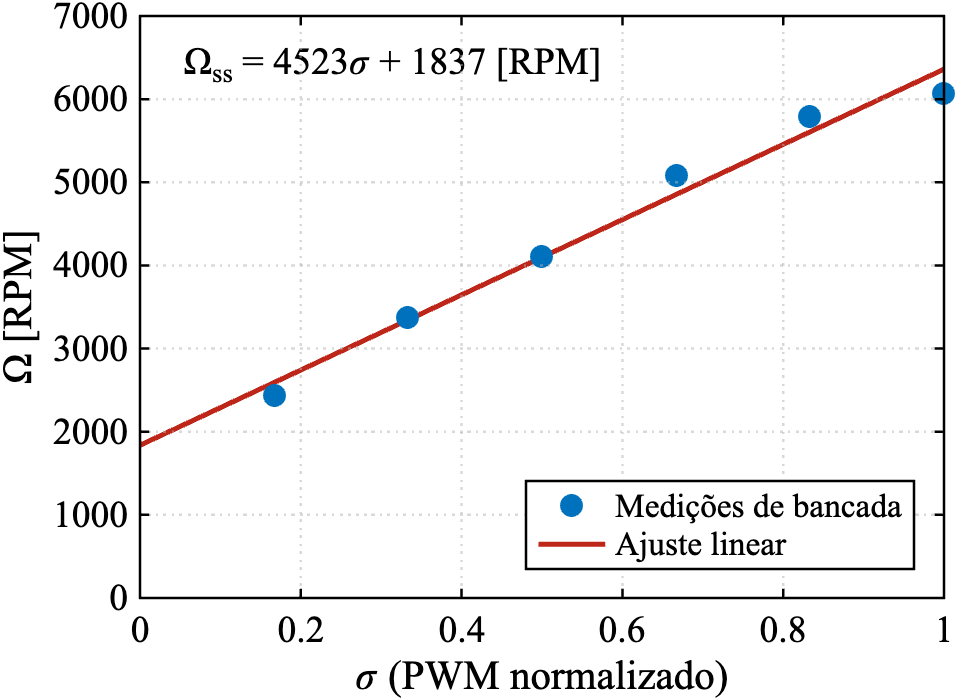
\includegraphics[width=0.78\textwidth]{ApeA/motor_pwm_rpm.png}
    \caption{Velocidade angular do rotor em regime permanente em função do comando normalizado. Os pontos são as medições de bancada e a linha contínua é o ajuste linear da Equação~\eqref{eq:motor-input}.}
    \label{fig:ap-pwm-rpm}
\end{figure}

O empuxo e o contra-torque de cada rotor crescem com o quadrado da velocidade angular, conforme as Equações~\eqref{eq:motor-thrust} e~\eqref{eq:motor-torque}. O ajuste quadrático aos dados de bancada, apresentado na Figura~\ref{fig:ap-tq}, fornece os coeficientes de referência $c_T = 1{,}76\times10^{-7}$~N/RPM$^2$ e $c_M = 5{,}04\times10^{-9}$~N$\cdot$m/RPM$^2$. A razão $c_M/c_T = 0{,}0286$~m, que aparece na linha de guinada da matriz de alocação (Equação~\eqref{eq:alocacao}), decorre diretamente desses dois ajustes.

\begin{figure}[ht]
    \centering
    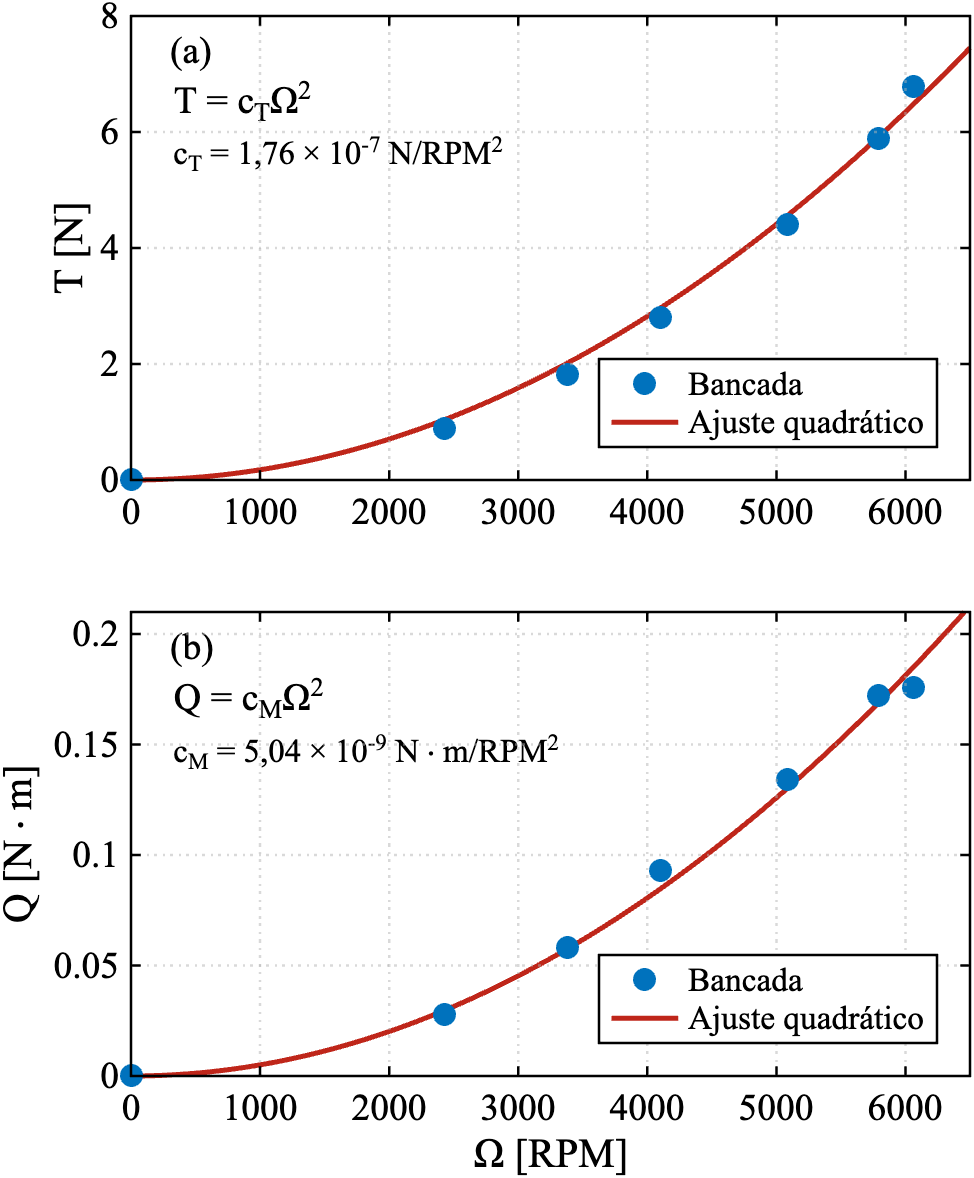
\includegraphics[width=0.8\textwidth]{ApeA/motor_thrust_torque.png}
    \caption{Empuxo (a) e contra-torque (b) em função da velocidade angular do rotor. Os pontos são as medições de bancada e as linhas contínuas são os ajustes quadráticos das Equações~\eqref{eq:motor-thrust} e~\eqref{eq:motor-torque}.}
    \label{fig:ap-tq}
\end{figure}

Por fim, a resposta do conjunto não é instantânea: a velocidade angular converge para o valor de regime com uma dinâmica de primeira ordem, de constante de tempo $\tau_m = 0{,}05$~s, considerada na reconstrução dos esforços a partir dos comandos PWM durante a identificação. Os coeficientes aqui obtidos servem de valor inicial; o empuxo e, sobretudo, o contra-torque de cada motor são reajustados individualmente na identificação por OEM (Capítulo~\ref{chap:resultados}), que absorve as diferenças entre os quatro atuadores e a maior incerteza associada à medição do contra-torque.

{\color{blue}
\section[{\color{blue}Estimativa das inclinações $k_v$ e $k_h$}]{{\color{blue}Estimativa das inclinações $k_v$ e $k_h$}}
\label{ap:kv-kh}

Os valores iniciais dos coeficientes de amortecimento angular das Equações~\eqref{eq:priori-lp} a~\eqref{eq:priori-nr} dependem das inclinações $k_v$ e $k_h$, calculadas nesta seção a partir do ponto de operação de pairado extraído da bancada. O empuxo de equilíbrio por rotor é $T_0 = mg/4 = 4{,}89$~N, ao qual a curva da Figura~\ref{fig:ap-tq} associa a rotação de pairado $\Omega_h \approx 5320$~RPM. Da teoria de quantidade de movimento, a velocidade induzida no pairado é $v_h = \sqrt{T_0/(2\rho A)} = 6{,}27$~m/s, em que $A$ é a área do disco da hélice \textit{slow flyer} 1045, de $10$ polegadas \cite{DeLucena2025}, e a razão de influxo resulta $\lambda_i = v_h/(\Omega_h R) \approx 0{,}089$.

A inclinação $k_v$ mede a variação do empuxo com a velocidade axial do cubo, o mecanismo do amortecimento por influxo \cite{Nguyen2025}, e decorre da combinação da quantidade de movimento com o elemento de pá:
\begin{equation}
  k_v = \frac{T_0}{v_h}\,\kappa, \qquad \kappa = \frac{a\,\sigma}{16\,\lambda_i + a\,\sigma},
  \label{eq:ap-kv}
\end{equation}
em que $\sigma = N_b\,c/(\pi R) \approx 0{,}125$ é a solidez da hélice de duas pás com corda média de $25$~mm e $a = 5$~rad$^{-1}$ é a inclinação de sustentação da seção, resultando $\kappa \approx 0{,}31$ e $k_v = 0{,}239$~N/(m/s). A inclinação $k_h$ mede a força no plano do disco por unidade de velocidade tangencial do cubo e sai do elemento de pá como
\begin{equation}
  k_h = \rho\,A\,(\Omega_h R)\,\frac{\sigma}{4}\left(C_{d0} + a\,\theta_{75}\,\lambda_i\right) = 0{,}0156~\text{N/(m/s)},
  \label{eq:ap-kh}
\end{equation}
com $C_{d0} = 0{,}03$ o arrasto de perfil da seção e $\theta_{75} \approx 10{,}8^{\circ}$ o passo geométrico a $75\%$ do raio. A corda média, a inclinação de sustentação e o arrasto de perfil da pá são hipóteses de projeto, de modo que esses valores carregam a incerteza típica de estimativas \textit{a priori}. Com os braços $\ell_y = 0{,}232$~m e $\ell_x = 0{,}327$~m e com $d^2 = \ell_x^2 + \ell_y^2$, as Equações~\eqref{eq:priori-lp} a~\eqref{eq:priori-nr} fornecem os valores iniciais $L_p = 0{,}0513$, $M_q = 0{,}1017$ e $N_r = 0{,}0100$~N$\cdot$m$\cdot$s, empregados no dimensionamento das manobras e como ponto de partida da identificação.
}

